%%%%%%%%%%%%%%%%%%%%%%%%%%%%%%%%%%%%%%%%%%%%%%%%%%%%%%%%%%%%%%%%%%%%%%%%
% Preamble
%%%%%%%%%%%%%%%%%%%%%%%%%%%%%%%%%%%%%%%%%%%%%%%%%%%%%%%%%%%%%%%%%%%%%%%%
\documentclass[11pt]{article}
%
% Packages and other includes
% Pagination
\usepackage[letterpaper, margin=1.25in]{geometry}
%
% Graphics, floats, tables
\usepackage{graphicx, color, float, array}
%
% Fonts
\usepackage[T1]{fontenc} % best for Western European languages
\usepackage{lmodern} % Latin Modern instead of CM
\usepackage{textcomp} % required to get special symbols
%
% Math
\usepackage{amsmath, amssymb}
\usepackage{braket}
%
% Hyperlinks
\usepackage{hyperref}
%
% Bibliography
\usepackage[style=numeric,sorting=none]{biblatex}
\addbibresource{references.bib}
%
% Revision (see Makefile)
\newcommand{\Revision}{977be36}

%
% Definitions and settings
% Paragraph indent and spacing
\setlength{\parskip}{0.4\baselineskip}
\setlength{\parindent}{0in}
%
% Math mode version of "r" column type (requires array package)
\newcolumntype{R}{>{$}r<{$}}
%
% Title, authors, date
\title{\textbf{Structures and Spectroscopy of Water-Halide Clusters}}
\author{Stan Laurel and Oliver Hardy}
\date{Chem 150L Winter 2018 \\ \today, Revision \Revision}
%
%
%%%%%%%%%%%%%%%%%%%%%%%%%%%%%%%%%%%%%%%%%%%%%%%%%%%%%%%%%%%%%%%%%%%%%%%%
% Main document
%%%%%%%%%%%%%%%%%%%%%%%%%%%%%%%%%%%%%%%%%%%%%%%%%%%%%%%%%%%%%%%%%%%%%%%%
%
\begin{document}

\maketitle

\begin{abstract}
  \noindent The abstract should contain a concise summary of the
  question/hypothesis investigated (first sentence), state the methods
  that were used to address it (second sentence), followed by a summary
  of the most important results (1-2 sentences), and the main
  conclusions (1-2 sentences). The abstract should be written in present
  tense.
\end{abstract}

\section{Introduction}

The first paragraph of the introduction should explain the broader
context of the computational experiment (1-2 sentences) and then
funnel the reader towards the research hypothesis/question posed in the
lab assignment.

In the second paragraph any relevant existing work in the literature should
be referenced, and the relation of this work to the current paper needs
to be stated and explained. An original research paper needs to present
something new and significant, and explain how its content goes beyond
existing work; for a lab report this paragraph can just state key
references and sources.

\section{Methods}

\subsection{Statement of the Models}

This section introduces theoretical models, equations, assumptions,
approximations, etc. that define the theoretical and computational
methodology. The section should contain enough information for the paper
to be self-contained, no more and no less. Existing methods
that have been extensively described elsewhere should not be discussed
in detail. For example, it is not recommended to derive the Hartree-Fock
equations here.

Symbols or mathematical operators should always be in math mode. Within
a text paragraph, use \$. For example, the electron charge is $e$, not
e, etc. Simple equations should be typeset using the equation
environment, e. g.,
\begin{equation}
  \label{eq:tdse}
  i \frac{ \partial}{\partial t} \ket{\Psi(t)} = \hat{H} \ket{\Psi(t)}.
\end{equation}
Equations are always a part of complete sentences, with proper
punctuation. Separating equations from text by colon or large arrays of
equations disconnected from the text should be avoided. All mathematical
symbols need to be defined, for example, in Eq. \eqref{eq:tdse},
$\hat{H}$ could denote the electronic Hamiltonian, and $\ket{\Psi}$ the
time-dependent electronic state.

\subsection{Computational Details}

Here is an example of a computational details section from a recent
paper \cite{Johannson14JPhysChemC118p29370}:

\begin{quote}
A global search of the potential energy surfaces of clusters with 9 to 13
gold atoms was performed using a genetic algorithm (GA)
\cite{Hartke.B:ACIE.2002, Johnston.R:DT.2003} based on the formulation by
Deaven and Ho \cite{Deaven.D:PRL.1995} as implemented in {\sc Turbomole}
\cite{Sierka.M:ACIE.2007}. The potential energy surfaces were evaluated at
the TPSS (meta-GGA) level \cite{Tao.J:PRL.2003} with polarized double-zeta
quality def2-SVP basis sets \cite{Weigend.F:PCCP.2005, Weigend.F:PCCP.2006}
and the Stuttgart-K\"{o}ln 1990 effective core potential (ECP) with 19
valence electrons \cite{Andrae.D:TCA.1990}. The resolution of the identity
approximation for the Coulomb energy (RI-\textit{J} method) was used
throughout \cite{Eichkorn.K:CPL.1995}. The GA optimizations were assumed to
be converged if no new minimum structures occurred among the lowest-energy
isomers during a certain number of generations. Another indicator of
convergence was the presence of both enantiomers for chiral structures. For
each cluster size, on the order of 1000 geometry optimizations were necessary
to converge the GA search. However, even for
extensive GA searches, there is no guarantee that the global minimum is found
in a finite number of steps. For completeness, simulated annealing
\emph{ab-initio} molecular dynamics simulations \cite{Elliott00a} were also
performed, but did not generate lower energy structures and failed to
find several of the low-energy structures obtained from the GA search.

The thus obtained low-energy structures were subsequently re-optimized at the
TPSS level using the triple-zeta quality 7s5p3d1f basis set specifically
devised for gold clusters \cite{Gilb.S:JCP.2002}. For Au$_{11}$, this
shortened bond lengths by 2-3 pm but did not qualitatively alter the
relative isomer energies. All optimized structures were confirmed to
be minima by analytical second derivative calculations 
\cite{Deglmann04a, vanWullen.C:JCC.2011}. Zero-point vibrational energies and
thermal corrections were evaluated using the rigid rotor--harmonic oscillator
approximation, after adjusting any very low-energy vibrations ($< 10$
cm$^{-1}$) to 10 cm$^{-1}$.

Final relative energies were obtained from single-point calculations at the
converged TPSS/7s5p3d1f structures using all-electron quadruple-zeta quality
QZ4P Slater-type basis sets \cite{vanLenthe.E:JCC.2003}, augmented by two
diffuse functions, obtained by dividing the smallest existing $s$ and $p$
exponents by 3.5; these basis sets will be denoted QZ4P(+sp). In the
all-electron calculations, relativistic effects were included using
the zeroth-order regular approximation (ZORA) \cite{Chang.C:PS.1986,
  vanLenthe:JCP.1993} and non-collinear spin-orbit (SO) corrections
\cite{Eschrig.H:JCC.1999}. Single-point all-electron ZORA calculations were
also performed with the revTPSS meta-GGA functional \cite{Perdew.J:PRL.2009}.
revTPSS restores the second-order gradient expansion for exchange and
produces accurate jellium surface energies. It thus resembles PBEsol
\cite{Perdew.J:PRL.2008}, which significantly outperforms the original PBE
GGA \cite{Perdew.J:PRL.1996} and rivals the good performance of TPSS for the
2D-3D transition in gold cluster anions \cite{Johansson.M:PRA.2008,
Johansson.M:JPCC.2008}. For the Au$_{12}^-$ anion, single point energies were
also computed with the M06-L functional \cite{M06-L}.

\end{quote}

For a lab report, this section can be shorter, but it needs to enable
an informed reader to reproduce the results. As opposed to other
sections, which are best written in present tense, the computational
details section should be in simple past.

\section{Results}

This section should report all results relevant to the
hypothesis/question introduced above. Rather than supplying ``commented
Gaussian output'' or all raw data, the section must be structured and
discuss the data in an intelligible way. Smaller data sets (up to $\sim$ 20
entries) are best reported as tables, larger and multivariate data sets
are best reported as figures. 

Tab. \ref{tab:ionE} is a slightly modified example from
Ref. \cite{Johannson14JPhysChemC118p29370}. Rules and other lines should be used
sparingly. Columns containing numerical data should be in math mode to
ensure, e.g., that minus signs are displayed as $-$, not - (dash). The
caption defines the data shown in all 
columns, including their units, and is relatively self-contained. Thus,
a reader with much background knowledge can retrieve important
information quickly by just reading the abstract and the tables,
figures, and their captions. Separate table or figure notes are best
avoided if possible, but if you need to use them, they may be generated
by enclosing the float into a minipage environment and using the
footnote command.

\begin{table}[htbp]
\label{tab:ionE}
\begin{tabular}{rclRRRRR}
  & 2D?    &        & \text{PBEsol} & \text{TPSS}  &
  \text{RPA}  & \text{revTPSS}  & \Delta G (100K) \\ 
  \hline
  Au$_8^+$-I    &       & $C_{2v}$ &    0   &   0   &   0   &   0     &   0
  \\
  II    &       &$ C_{s} $ &  +7.1  &  +2.4 &  +0.7 & +10.2   &  +8.1
  \\
  III   & $\surd$ & $D_{2h}$ & +16.7 &  +8.7 & +17.4 & +26.4   & +24.6 
  \\
  IV    & $\surd$ & $C_{2v}$ & +17.8  & +12.7 & +11.3 & +27.1   & +23.8
  \\
  \hline
  Au$_{12}^-$-I &      & $C_{2v}$ &   0    &   0   &   0   &   0    &  0
  \\  
  II & $\surd$ &$ D_{3h}$ &  -9.1  & -19.5 &  -6.8 &  +1.9   & +1.0  \\   
  \hline
\end{tabular}

\caption{Dimensionalities, point groups, relative energies 
at 0 K (kJ/mol) between the energetically lowest 2D and 3D structures
for Au$_8^+$ and Au$_{12}^-$; all relative energies include the
vibrational zero-point-energy and spin-orbit coupling, the computed free
energy differences $\Delta G$(100K) are based on revTPSS electronic
energies.} 
\end{table}

When making figures, vector graphics (svg, eps, and native pdf formats)
is always preferable for simple plots and diagrams, because it allows
scaling without quality loss. For images, complex molecular
visualizations such as orbital plots or rendered molecular graphics,
bitmaps such as png or jpg are used. 

Fig. \ref{fig:hloss} shows an example from
\cite{Vincent16JPhysChemLett7p4185} containing vector graphics figures.
\begin{figure}[htbp]
  \centering
  \label{fig:hloss}

  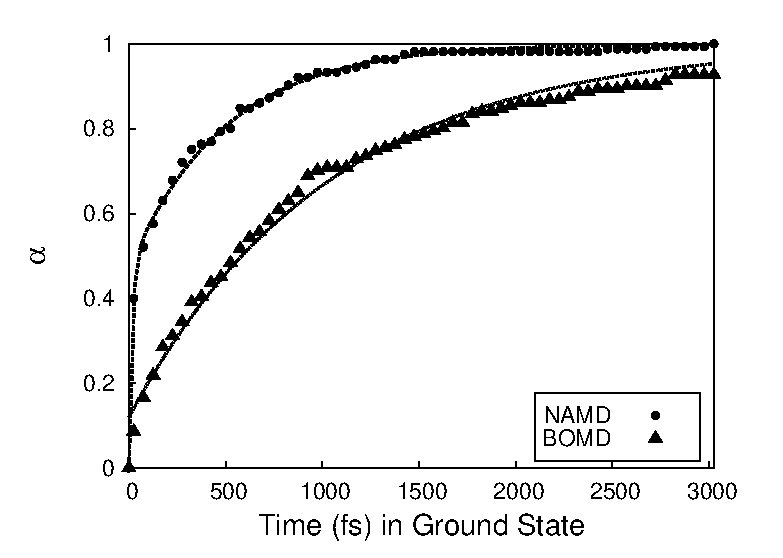
\includegraphics[width=.49\textwidth]{decay.eps}
  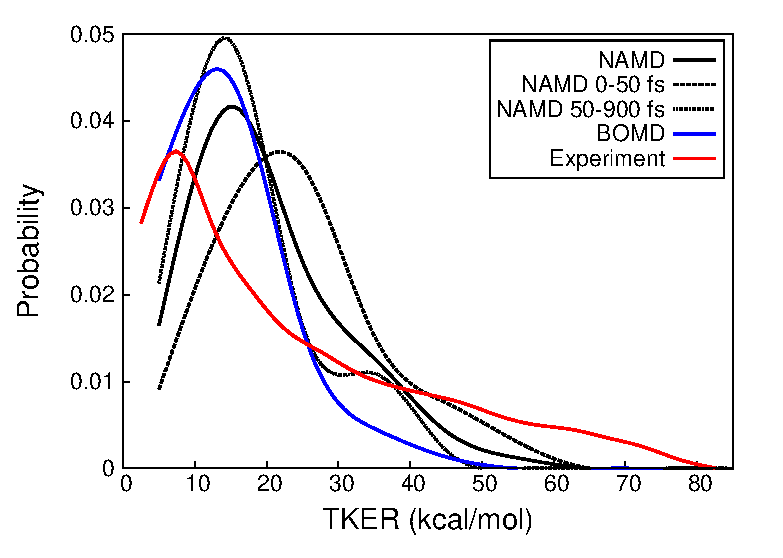
\includegraphics[width=.49\textwidth]{namdbomdall.eps}

  \caption{(a) Degree of C--H dissociation $\alpha$ for
    channels (1)--(3) as a function of time spent in the S$_0$ 
    state. Grey dotted curves indicate mono- (BOMD) and biexponential
    (NAMD) fits. (b) Comparison of the experimental TKER probability
    distributions \cite{Lee09JChemPhys131p174312} (purple) for the
    H-loss channels (1)-(3) to BOMD (blue) and NAMD (gray)
    simulations. The NAMD TKER distribution is the sum of TKER
    resulting from fast (0-50 fs) and slow (50-3000 fs) dissociations.}  
\end{figure}
The optional width argument of the includegraphics command allows
specification of the figure width while keeping the aspect ratio. 

It is not recommended to ``pin'' floats such as tables and figures to
certain places in the text. Rather, the optional arguments of the table
or figure environment should be used to specify the preferred alignment
(in order of priority), e.g., h for ``here'', t for ``top'', b for
bottom of a page, and p for a separate page containing floats only.

The text may guide the reader through the results and discuss them, but
should not merely re-state the contents of the tables and figures.


\section{Conclusions}

This section should aim to answer the hypothesis or question stated in
the introduction clearly and concisely, as well as other possibly
significant results of the study. Do not provide a summary of your work
here, the correct place for that is the abstract. Instead, the
conclusions must explain what has been learned, and how it is relevant to the
initial question.

\section*{Acknowledgments}

This section should acknowledge any additional sources of support from
professionals who aren't co-authors but helped you complete your work. For
example, O. H. would like to acknowledge useful discussions with The
Three Stooges. Often, funding agencies mandate that funding be
acknowledged in this section. 

\printbibliography

\end{document}
